
\chapter{Cadre g\'{e}ng\'{e}rale du projet}

\section{Introduction}

 Au cours de ce chapitre, nous allons nous int\'{e}resser par la
pr\'{e}sentation du contexte du travail ainsi que la pr\'{e}sentation de Start up
Cherchini pour laquelle ce travail a \'{e}t\'{e} r\'{e}alis\'{e}.
Puis on passe par la th\'{e}matique du projet dans laquelle on va indiquer la
probl\'{e}matique, citer des produits existants sur le march\'{e}, sp\'{e}cifier les besoins
et indiquer la solution propos\'{e}e. Ainsi qu'on va d\'{e}crire la m\'{e}thodologie avec
laquelle on a pu concevoir et r\'{e}aliser notre projet, et on finit par la
pr\'{e}sentation de l'architecture de projet tout en en expliquant les choix
techniques et les outils n\'{e}cessaires.


\section{Contexte du travail}

 Ce stage s'inscrit dans le cadre d'un projet de fin d'\'{e}tudes pour l'obtention du
dipl\^{o}me Ing\'{e}nieur en informatique De l'Ecole Sup\'{e}rieure Priv\'{e}e des
Technologies de l'Information et de Management de Nabeul.

 Notre stage a \'{e}t\'{e} effectu\'{e} au sein de Start up Cherchini.
Le sujet est intitul\'{e} \guillemotleft{}Cr\'{e}ation d'une plateforme de gestion des projets\guillemotright{}




\section{Pr\'{e}sentation  de l'organisme d'accueil}

\bigskip
 Cherchini.tn est une agence de communication, cr\'{e}e en 2017, qui vous aide \`{a}
d\'{e}finir vos objectifs afin de vous fournir la solution web la plus adapt\'{e}e \`{a} vos
besoins. Cherchini.tn cherche souvent d'\^{e}tre \`{a} la pointe de l'innovation par sa
cr\'{e}ation graphique (logos, chartes graphiques, banni\`{e}res publicitaires,..),
cr\'{e}ation web, web design et r\'{e}f\'{e}rencement des sites web.

\bigskip
 En outre, Cherchini.tn vous offre des solutions de vente en ligne, son objectif
est de mettre en relation les clients et les vendeurs dans le but de r\'{e}aliser de
tr\`{e}s bonnes affaires tout en b\'{e}n\'{e}ficiant de ses expertises.

Site Web : https://cherchini.tn/

\bigskip

  \FloatBarrier
\begin{figure}[H]
\center

\includegraphics[width=10cm,height=9cm]{./figures/cherchini-logo.png}
\caption{Logo de Cherchini.}

\end{figure}
  \FloatBarrier

\section{ Contexte du projet }
Ce stage s'inscrit dans le cadre d'un projet de fin d'\'{e}tudes pour l'obtention du
dipl\^{o}me Ing\'{e}nieur en informatique De l'Ecole Sup\'{e}rieure Priv\'{e}e des
Technologies de l'Information et de Management de Nabeul.
Notre stage a \'{e}t\'{e} effectu\'{e} au sein de Start up Cherchini.
Le sujet est intitul\'{e} \guillemotleft{}Cr\'{e}ation d'une plateforme de gestion des projets\guillemotright{}

\section{Business intelligence}
 L'informatique d\'{e}cisionnelle, aussi appel\'{e}e business intelligence(BI), d\'{e}signe un ensemble de m\'{e}thodes, de moyens et d'outils informatiques utilis\'{e}s pour piloter une entreprise et aider \`{a} la prise de d\'{e}cision : tableaux de bord, rapports analytiques et prospectifs.

\section{ Etude de l'existant  }
Il existes sur le march\'{e} plusieurs plateformes de gestion des projet , et parmi
les outils les plus connues on trouve ASANA et JIRA .

\subsection{Asana}

Il s'agit d'une plate-forme robuste qui sert \`{a} vos \'{e}quipes de rester concentr\'{e}es
sur les objectifs, les projets et les t\^{a}ches quotidiennes .Voici les
fonctionnalit\'{e}s les plus importantes qu'elle offre :


\begin{itemize}
\item{Tableau de bord permet de visualiser facilement votre travail.}

\item{ Voir la grande image. Clouez votre timing en visualisant les travaux sur
un calendrier. Rep\'{e}rez facilement les trous et les chevauchements dans
votre horaire et effectuez rapidement les ajustements n\'{e}cessaires.}

\item{Gardez une trace de ce qui est le plus important.}

\item{Pas besoin de r\'{e}inventer la roue. Transformez les processus courants en
mod\`{e}les que votre \'{e}quipe enti\`{e}re peut utiliser pour que les projets se
d\'{e}roulent sans heurts \`{a} chaque fois.}

\item{Partagez des informations avec les bonnes personnes. Rendez les
\'{e}quipes et les projets priv\'{e}s afin de cr\'{e}er un espace s\'{e}curis\'{e} pour les
travaux sensibles.}

\item{Partagez des informations avec les bonnes personnes. Rendez les
\'{e}quipes et les projets priv\'{e}s afin de cr\'{e}er un espace s\'{e}curis\'{e} pour les
travaux sensibles.}

\end{itemize}

\subsection{Jira}
Qui est l'un des meilleurs outils de gestion de produit qui comprend :
\begin{itemize}

\item{Le suivi et la gestion des probl\`{e}mes}

\item{La gestion des produits}

\item{Un Tableau de bord configurable}

\item{Des Rapport sur l'avancement du projet}

\item{Support des m\'{e}thodologies Scrum \& Kanban}

\end{itemize}



\section{ Probl\'{e}matique }
Toute entreprise aspire \`{a} se conformer au triangle d'or (D\'{e}lai, Cout, Qualit\'{e})
autour du quel tournent tous les projets professionnelles.




Dans le but d'organiser ses projets, Cherchini veut r\'{e}aliser son propre outil de
gestion des projets, en fait, l'absence d'un tel outil demeurent inaper\c{c}ue
pour les premi\`{e}res ann\'{e}es d'une nouvelle entreprise et surtout pour les
petites ou moyenne entreprises, mais \'{e}videmment, cela va engendrer au futur
une mal organisation et une perte des informations importantes, et en
cons\'{e}quence une perte de temps et d'argent.

On remarque alors que les outils existants sont assez sophistiqu\'{e}s.
Ainsi que ces deux outils, ils existent plusieurs concurrents qui offrent
plusieurs manipulations et possibilit\'{e}s.
Les fonctionnalit\'{e}s sont payantes pour chacun de ces outils et Cherchini n'a
pas besoin de tous ces fonctionnalit\'{e}s d'une part, et d'autre part elle voudrait
\^{e}tre capable d'\'{e}tendre certaines fonctionnalit\'{e}s et de les r\'{e}duire selon le
besoin .Par exemple, ajouter une carte g\'{e}ographique qui indique la
g\'{e}olocalisation de ses partenaires dans cette plateforme .
Pour cela, Cherchini voudrais avoir son propre outil de gestion de projet et d\'{e}sire r\'{e}aliser un
service d'informatique d\'{e}cisionnelle (Business Intelligence) ,ce service doit donner une vue g\'{e}n\'{e}rale sur le d\'{e}roulement des projets
selon les couts et les d\'{e}lais \`{a} suivre.


\begin{figure}[H]
\center
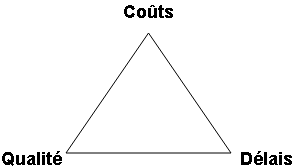
\includegraphics[width=8cm,height=5cm]{./figures/triangle.png}
\caption{Triangle d'or.}
\end{figure}




\section{ Solution propos\'{e}e  }
Pour r\'{e}pondre aux besoins fonctionnels, nous avons construit une application web en
se basant sur l’architecture suivante.


\begin{figure}
\center
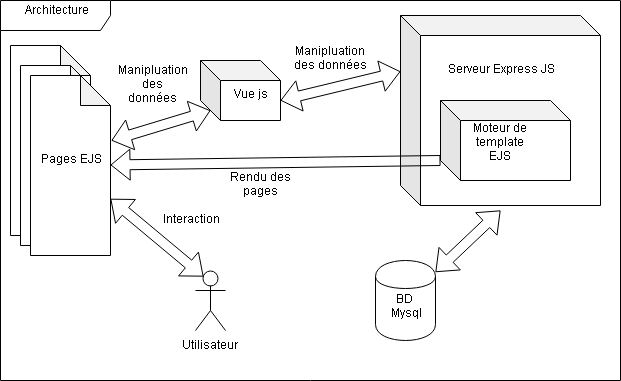
\includegraphics[width=10cm,height=10cm]{./figures/archi.png}
\caption{Architecture g\'{e}n\'{e}rale.}
\end{figure}

Comme nous avons indiqu\'{e}, pour \^{e}tre capable d'\'{e}tendre les fonctionnalit\'{e}s
selon le besoin en \'{e}vitant la complexit\'{e} des outils existantes et les couts de
paiement pour chaque fonctionnalit\'{e}, on a adopt\'{e} des technologies open
sources et gratuits, et voici les technologies qu'on a utilis\'{e} :
\begin{itemize}
\item{Pour la base de donn\'{e}es : MYSQL}
\item{Pour le serveur et API REST : Express JS ,NODE JS}
\item{Moteur de Template (engine view) : EJS }
\item{Pour les pages web : HTML et Vue js}
\item{Pour l'authentification : JWT }
\item{Pour la carte de g\'{e}olocalisation des clients : LeafLet maps}
\item{Pour le diagramme de Gantt et les rapport : Highcharts}

\end{itemize}

\section{Etude foncionnelle et choix m\'{e}thodologique}


